%# -*- coding: utf-8 -*-
% !TeX encoding = UTF-8 Unicode
% !TeX spellcheck = en_US
% !TeX TS-program = xelatex
%~ \XeTeXinputencoding "UTF-8"
% vim:ts=4:sw=4
%
% 以上设定默认使用 XeLaTex 编译,并指定 Unicode 编码,供 TeXShop 自动识别
%\documentclass[dvipdfm]{beamer}  %dvipdfm选项是关键,否则编译统统通不过
\documentclass{beamer}

\newcommand{\doctitle}{mrnative -- Run your native code in any Hadoop environments}
\newcommand{\docauthor}{Yunhui Fu}
\newcommand{\dockeywords}{{HPC}{Hadoop}{map}{reduce}}
\newcommand{\docsubject}{}
\newcommand{\doczhcn}{}


\newcommand{\comments}[1]{}
%\renewcommand{\comments}[1]{#1}

%----------------------------------------------------------
% User packages

% the algorithm2e package
\makeatletter
\newif\if@restonecol
\makeatother
\let\algorithm\relax
\let\endalgorithm\relax
%%\usepackage[figure,ruled,vlined]{algorithm2e}
\usepackage[ruled,vlined]{algorithm2e}

\usepackage{ifthen}
\usepackage{ifpdf}
\usepackage{ifxetex}
\usepackage{ifluatex}
\ifxetex % xelatex
\else
    %The cmap package is intended to make the PDF files generated by pdflatex "searchable and copyable" in acrobat reader and other compliant PDF viewers.
    \usepackage{cmap}%
\fi

% 用于接受从 xelatex/pdflatex 通过参数 -jobname 传入的参数来判定编译何种语言的版本。
% \cnt 的三个参数分别为 en/zh/tw 的内容
\newcommand{\cnt}[3]{{#1}{#2}{#3}}
%\newcommand{\cnt}[3]{#1} % default en
\usepackage{ifthen}
\ifthenelse{\equal{\detokenize{lang-zh}}{\jobname}}{
  \renewcommand{\cnt}[3]{#2}
}{
  \ifthenelse{\equal{\detokenize{lang-tw}}{\jobname}}{
    \renewcommand{\cnt}[3]{#3}
  }{
    % default en
    \renewcommand{\cnt}[3]{#1}
  }
}

% 根据配置来设置中文环境
\newcommand{\zhenv}[1]{}
\cnt{}{\renewcommand{\zhenv}[1]{#1}}{\renewcommand{\zhenv}[1]{#1}}

\zhenv{
\usepackage{ifxetex}
%------------------------------------------------------------------------------------------------------
%U no, it's happy to use chinese now.
%需要注明的是,这种方法是我暂时惟一发现中文XeLaTeX对moderncv原样支持的方式。
%另外几种方式,我得花时间再去试一下,有很多问题,应该只是宏包的冲突。
% 2009-10-3 3:41:57 Saturday
%~ \usepackage{xltxtra,fontspec,xunicode}    %Xelatex支持
%~ \usepackage{zhfont}                       %用zhspacing包支持,之后我再去看 另一种实现是否有问题。
%~ \zhspacing
%\usepackage{xltxtra,xunicode}

\ifxetex % xelatex
    %% chinese setup
    \usepackage[cm-default]{fontspec} % XeLaTex 配合 fontspec 可以非常方便地設置字體。 [cm-default] 選項主要用來解決使用數學環境時數學符號不能正常顯示的問題
    \usepackage{xltxtra,xunicode} % 這行和上行 \usepackage[cm-default]{fontspec} 解決公式不正常的問題.但是打開後有些如 itemize 的點不能顯示。

    \usepackage[
        BoldFont,   % 允許粗體
        SlantFont,  % 允許斜體
        %CJKsetspaces,
        CJKchecksingle
        ]{xeCJK}
    \defaultfontfeatures{Mapping=tex-text} %如果沒有它,會有一些 tex 特殊字符無法正常使用,比如連字符。

    \XeTeXlinebreaklocale "zh" % 重要,使得中文可以正確斷行!
    \XeTeXlinebreakskip = 0pt plus 1pt minus 0.1pt

%----------------------------------------------------------------------------------------
% 以下四行是设置可能用到的字体,但若无其它设定,本文档所用之默认字体为
% $zhspacing/zhfont.sty文件中的第71行附近,关于zhsffont的定义
% \newfontfamilywithslant\zhsffont{Adobe Heiti Std R}
% 即以下四行配置无实际作用。zhfont中设定优先级更高。
% zhspacing文档的解释是对于XeLaTeX和XeLaTeX对应的宏方案不同。
% 亦不支持\font\myname={"SuSE"}型宏。
    %\setCJKmainfont[BoldFont={WenQuanYi Micro Hei}]{AR PL UMing CN}
    %\setCJKsansfont{AR PL UMing CN} %{Microsoft YaHei}
    %\setCJKmonofont{WenQuanYi Micro Hei Mono}
    \setCJKmainfont[BoldFont={Adobe Heiti Std}, ItalicFont={Adobe Kaiti Std}]{Adobe Song Std}
    \setCJKsansfont{Adobe Ming Std} %{AR PL UMing CN} %{Microsoft YaHei}
    \setCJKmonofont{Adobe Fangsong Std}

    \setmainfont{Times New Roman}
    \setsansfont{DejaVu Sans}
    \setmonofont{FreeMono}%{Latin Modern Mono}
    %\setsansfont{[foo.ttf]} % 直接使用当前目录下的字体文件

%~ \setmainfont{Scala}           %英文字体
%~ \setmonofont{Nimbus Sans L}                     %英文等宽体
%~ \setsansfont[BoldFont={Myriad Pro}]{Myriad Pro}    %不注释了 线性非线性,这边没有限制。
%----------------------------------------------------------------------------------------
% 当然,可以在文本档第14行处,将roman/san 选项换一下,就可以更换main字体了,
% 但这并不能改变全文字体单调的囧境。
% 2009-10-3 3:44:41 Saturday
%一个折衷的方案,另定义字体宏。
%~ \usepackage{fontspec}  

%~ \newfontfamily\ni{"SimHei"}

    \defaultfontfeatures{Mapping=tex-text}
\fi
} % \zhenv

\usepackage{tabularx} % long table
\usepackage{booktabs,longtable} % table in seperate pages.

% ============================================
% Check for PDFLaTeX/LaTeX
% ============================================
\newcommand{\outengine}{xetex}
\newif\ifpdf
\ifx\pdfoutput\undefined
  \pdffalse % we are not running PDFLaTeX
  \ifxetex
    \renewcommand{\outengine}{xetex}
  \else
    \renewcommand{\outengine}{dvipdfmx}
  \fi
\else
  \pdfoutput=1 % we are running PDFLaTeX
  \pdftrue
  \usepackage{thumbpdf}
  \renewcommand{\outengine}{pdftex}
\fi
\usepackage{hyperref}
\hypersetup{\outengine,
    bookmarksnumbered, %dvipdfmx
    %% unicode, %% 不能有unicode选项,否则bookmark会是乱码
    colorlinks=true,
    urlcolor=blue,        % \href{...}{...} external (URL)
    filecolor=red,      % \href{...} local file
    linkcolor=black, % \ref{...} and \pageref{...}
    breaklinks,
    pdftitle={\doctitle},
    pdfauthor={\docauthor},
    pdfsubject={\docsubject},
    pdfkeywords={\dockeywords},
    pdfproducer={Latex with hyperref},
    pdfcreator={pdflatex},
    %%pdfadjustspacing=1,
    pdfborder=1,
    pdfpagemode=None,
    pagebackref,
    bookmarksopen=true
}

\usepackage{makeidx}       	% Package to make an index.
\makeindex    % Make the index

\usepackage{amssymb}
\usepackage{amsmath,amsthm,amsfonts,amscd} 

%\usepackage[margin=2.5cm,nohead]{geometry}

\usepackage{color}

\definecolor{darkgreen}{rgb}{.2,.5,.2}
\definecolor{grey}{rgb}{.9,.9,.9}
\definecolor{red}{rgb}{1,0,0}
\definecolor{olive}{rgb}{.2,.5,.3}
\definecolor{CadetBlue}{cmyk}{0.62,0.57,0.23,0}
\definecolor{OliveGreen}{cmyk}{0.64,0,0.95,0.40}

\usepackage{tabularx} % long table
\usepackage{booktabs,longtable} % table in seperate pages.
\usepackage{array}
% table's multirow and multicolumn
\usepackage{multirow}

% Setup TikZ
\usepackage{tikz}
\usetikzlibrary{shapes} % ecllipse
\usetikzlibrary{arrows}
\tikzstyle{block}=[draw opacity=0.7,line width=1.4cm]

\definecolor{darkgrey}{rgb}{.66,.66,.66}
\definecolor{cyan}{rgb}{0,1,1}
\definecolor{deeppink}{rgb}{1,.08,.57}
\definecolor{rosybrown}{rgb}{.73,.56,.56}
\definecolor{firebrick}{rgb}{.69,.13,.13}

% --------------------------------------------
% Load graphicx package with pdf if needed 
% --------------------------------------------
\ifxetex    % xelatex
    \usepackage{graphicx}
\else
    \ifpdf
        \usepackage[pdftex]{graphicx}
        \pdfcompresslevel=9
    \else
        \usepackage{graphicx} % \usepackage[dvipdfm]{graphicx}
    \fi
\fi
%% \DeclareGraphicsRule{.jpg}{eps}{.bb}{}
%\DeclareGraphicsRule{.png}{eps}{.bb}{}
\graphicspath{{../figures/} {figures/}}
\usepackage{flafter} % 防止图形在文字前


\usepackage{chapterbib}

\usepackage{courier}
\usepackage{listings} % list the source code
\definecolor{ForestGreen}{rgb}{0.13,0.55,0.13}

\lstset{
    language=C,
    captionpos=b, %t,
    tabsize=3,
    basicstyle=\footnotesize\ttfamily, %basicstyle=\ttfamily\normalsize, %basicstyle=\small\ttfamily, %\normalfont\ttfamily, % \large\ttfamily, % \small\ttfamily, % \footnotesize\ttfamily, % \scriptsize\ttfamily, % Standardschrift,
    numbers=left,               %左侧显示行号 往左靠,还可以为right,或none,即不加行号
    stepnumber=1,               %若设置为2,则显示行号为1,3,5,即stepnumber为公差,默认stepnumber=1
    %numberstyle=\tiny,         %行号字体用小号
    numberstyle={\color[RGB]{0,192,192}\tiny} ,%设置行号的大小,大小有tiny,scriptsize,footnotesize,small,normalsize,large等
    numbersep=8pt,              %设置行号与代码的距离,默认是5pt
    breaklines=true,            %对过长的代码自动换行
    showstringspaces=false,     %不显示代码字符串中间的空格标记
    frame=shadowbox, %=lines,                    %把代码用带有阴影的框圈起来
    stringstyle=\ttfamily,      % 代码字符串的特殊格式
    commentstyle=\color{ForestGreen}, %\color{red!50!green!50!blue!50}, %浅灰色的注释
    rulesepcolor=\color{red!20!green!20!blue!20}, %代码块边框为淡青色
    keywordstyle=\color{blue!90}\bfseries,        %代码关键字的颜色为蓝色,粗体
    backgroundcolor=\color[rgb]{1,1,1},%\color[RGB]{245,245,244},   %代码背景色 \color[rgb]{0.91,0.91,0.91}
    framextopmargin=2pt,framexbottommargin=2pt,abovecaptionskip=-3pt,belowcaptionskip=3pt,
%    xleftmargin=4em,xrightmargin=4em, % 设定listing左右的空白
%    %language={[ISO]C++},       %language为,还有{[Visual]C++}
%    alsolanguage=Java,
%    %alsolanguage=[ANSI]C,      %可以添加很多个alsolanguage,如alsolanguage=matlab,alsolanguage=VHDL等
%    %alsolanguage= tcl,
%    alsolanguage= XML,
%    keepspaces=true,            %
%    breakindent=22pt,           %
%    breakindent=4em,            %
%    showspaces=false,           %
%    flexiblecolumns=true,       %
%    breakautoindent=true,       %
%    aboveskip=1em,              %代码块边框
%    %% added by http://bbs.ctex.org/viewthread.php?tid=53451
%    fontadjust,
%    texcl=true,
%    escapeinside=``,            %在``里显示中文
%    %escapebegin=\begin{CJK*}{GBK}{hei},escapeend=\end{CJK*},
%    % 设定中文冲突,断行,列模式,数学环境输入,listing数字的样式
%    extendedchars=false,columns=flexible,
%    mathescape=false,
%    % numbersep=-1em,
    emph={label}
}

\renewcommand{\ttdefault}{pcr}

\definecolor{darkgreen}{cmyk}{0.7, 0, 1, 0.5}
\definecolor{darkblue}{rgb}{0.1, 0.1, 0.5}
\lstdefinelanguage{diff}
{
    keywords={+, -, \ , @@, diff, index, new},
    sensitive=false,
    morecomment=[l][""]{\ },
    morecomment=[l][\color{darkgreen}]{+},
    morecomment=[l][\color{red}]{-},
    morecomment=[l][\color{darkblue}]{@@},
    morecomment=[l][\color{darkblue}]{diff},
    morecomment=[l][\color{darkblue}]{index},
    morecomment=[l][\color{darkblue}]{new},
    morecomment=[l][\color{darkblue}]{similarity},
    morecomment=[l][\color{darkblue}]{rename},
}

\lstdefinelanguage{JavaScript}{
  keywords={typeof, new, true, false, catch, function, return, null, catch, switch, var, if, in, while, do, else, case, break},
  keywordstyle=\color{blue}\bfseries,
  ndkeywords={class, export, boolean, throw, implements, import, this},
  ndkeywordstyle=\color{darkgray}\bfseries,
  identifierstyle=\color{black},
  sensitive=false,
  comment=[l]{//},
  morecomment=[s]{/*}{*/},
  %commentstyle=\color{purple}\ttfamily,
  commentstyle=\color{green}\ttfamily,
  stringstyle=\color{red}\ttfamily,
  morestring=[b]',
  morestring=[b]"
}

%----------------------------------------------------------
%%%%%%%%%%%%%%%%%%%%%%%%%%%%%%%%%%%%%%%%%%%%%%%%%%%%%%%%%%%%%%%%%%%%%%
%	Some math support.					     %
%%%%%%%%%%%%%%%%%%%%%%%%%%%%%%%%%%%%%%%%%%%%%%%%%%%%%%%%%%%%%%%%%%%%%%
%
%	Theorem environments (these need the amsthm package)
%
%% \theoremstyle{plain} %% This is the default

\newtheorem{thm}{Theorem}[section]
\newtheorem{cor}[thm]{Corollary}
\newtheorem{lem}[thm]{Lemma}
\newtheorem{prop}[thm]{Proposition}
\newtheorem{ax}{Axiom}

\theoremstyle{definition}
\newtheorem{defn}{Definition}[section]

\theoremstyle{remark}
\newtheorem{rem}{Remark}[section]
\newtheorem*{notation}{Notation}

%\numberwithin{equation}{section}


%----------------------------------------------------------

\usepackage{fontspec,xunicode,xltxtra}

%\usepackage{beamerthemesplit}
\usetheme{Madrid}
%\usetheme{PaloAlto}
%\usetheme{Warsaw}
%\usetheme{Luebeck}
%\usetheme{Antibes}
%\usetheme{Darmstadt} %
%\usetheme{Copenhagen}

% Choose color scheme
%
%\usecolortheme{default}
%\usecolortheme{albatross}
%\usecolortheme{crane}

%\usecolortheme{sidebartab}
%\usecolortheme{beetle}
%\usecolortheme{dove}
%\usecolortheme{fly}
%\usecolortheme{seagull}
%\usecolortheme{lily}
%\usecolortheme{orchid}

%\setsansfont[Mapping=tex-text]{Adobe 黑体 Std}
    %% 如果装了Adobe Acrobat,可在font.conf中配置Adobe字体的路径以使用其中文字体
    %% 也可直接使用系统中的中文字体如SimSun,SimHei,微软雅黑 等
    %% 原来beamer用的字体是sans family;注意Mapping的大小写,不能写错
    %% 设置字体时也可以直接用字体名,以下三种方式等同:
    %\setromanfont[BoldFont={黑体}]{宋体}
    %\setromanfont[BoldFont={SimHei}]{SimSun}
    %\setromanfont[BoldFont={"[simhei.ttf]"}]{"[simsun.ttc]"}

\title{\sc{\doctitle}}
\author{\docauthor}
\date{Nov 25, 2015}

%\pgfdeclareimage[height=1.5cm]{logo}{./figures/TigerPaw_co.eps}
%\pgfdeclareimage[height=1.5cm]{logo}{../figures/cuseal.eps}
%\logo{\pgfuseimage{logo}}

%\institute[PhD]{Computer Science}
\subject{Talks}

\begin{document}

\frame{\titlepage}
\section*{Contents}%{大纲}
\frame{\tableofcontents}



\section{Introduction}

\frame {
    \frametitle{The mrnative stack}

\begin{figure}\centering
  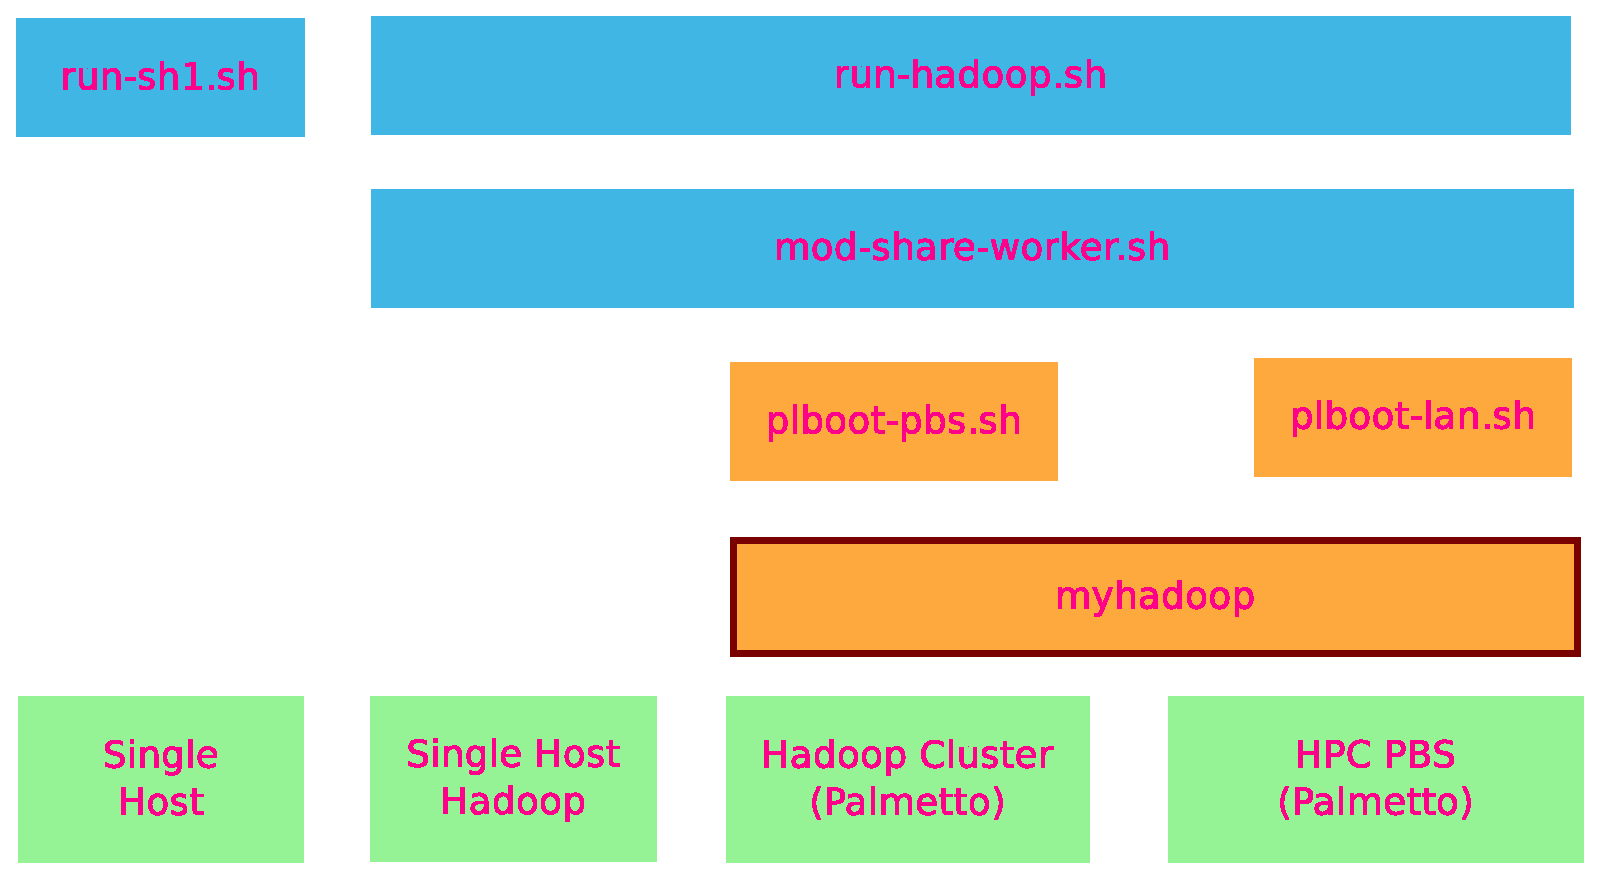
\includegraphics[width=0.8\textwidth]{mrnative-stack}
  \caption{The stack of the mrnative}\label{fig:mrnativestack}
\end{figure}

    \begin{itemize}
      \item write map/reduce code in native code
      \item run in various system settings
      \item supports single host, single host Hadoop, Hadoop cluster, and HPC PBS over myhadoop
    \end{itemize}
}




\section{Usage}

\begin{frame}[fragile]
  \frametitle<presentation>{single host}

    \begin{itemize}
      \item emulate the streaming mode map/reduce in bash;
      \item test the correctness of your process flows;
      \item run a small amount of tasks which can use all of the cores in the system;

      \item get the results in a subdir \texttt{output-*}
\begin{lstlisting}[language=bash]
cd projtools
./run-sh1.sh
\end{lstlisting}
    \end{itemize}

\end{frame}


\begin{frame}[fragile]
  \frametitle<presentation>{single host Hadoop}

    \begin{itemize}
      \item simulate a Hadoop environment;
      \item to find out Hadoop environment related problems;

      \item get the results in a HDFS \texttt{hdfs://tmp/\${USER}/output-*}
\begin{lstlisting}[language=bash]
cd projtools
./run-hadoop.sh
\end{lstlisting}
    \end{itemize}

\end{frame}



\begin{frame}[fragile]
  \frametitle<presentation>{Hadoop Cluser}

    \begin{itemize}
      \item run your program in a productive environment;
      \item run a huge amount of small tasks;
      \item you need to set two variables in your \texttt{mrsystem.conf}: (b/c we can't set the vcore mem parameters)
        \begin{itemize}
          \item \texttt{HDFF\_NUM\_CLONE} to 1.
          \item \texttt{HDFF\_TOTAL\_NODES} to the number of vcores (eg. 400); and
        \end{itemize}

      \item get the results in a HDFS \texttt{hdfs://tmp/\${USER}/output-*}
\begin{lstlisting}[language=bash]
ssh $USER@user.palmetto.clemson.edu
ssh resourcemgr.palmetto.clemson.edu
cd projtools
./run-hadoop.sh
\end{lstlisting}
    \end{itemize}

\end{frame}


\begin{frame}[fragile]
  \frametitle<presentation>{HPC PBS with myHadoop}

    \begin{itemize}
      \item run your program in a productive environment;
      \item run a huge amount of small tasks;
      \item automatically detects the available resources,
            and setup the required config files for Hadoop;

      \item get the results in the \texttt{/scratch1/\${USER}/output-*}
\begin{lstlisting}[language=bash]
ssh $USER@user.palmetto.clemson.edu
cd projtools
./run-hadooppbs.sh
\end{lstlisting}
    \end{itemize}

\end{frame}


\section{Configuration}


\begin{frame}[fragile]
  \frametitle<presentation>{Three type of config files}

    \begin{itemize}
      \item \texttt{mrsystem.conf} -- the configs for the software, such as the number of nodes, the scratch directory etc;
      \item \texttt{input/} or \texttt{input.conf} -- the configs for input data;
      \item \texttt{output/} or \texttt{output.conf} -- the configs for output data;
    \end{itemize}

\end{frame}



\section{Compile 3rd party tools}


\begin{frame}[fragile]
  \frametitle<presentation>{Compile 3rd party tools}

    \begin{itemize}
      \item using the compile scripts in folder \texttt{3rd};
      \item current version supports compiling \texttt{ns2, ffmpeg, opencv}, and gnu tools such as \texttt{gawk, gnuplot} etc.;
      \item the compiled binaries are packed in a \texttt{tar.gz} file;
      \item the \texttt{tar.gz} package contains the required libraries and support files, strip other redunant binaries or files generated during compiling;
    \end{itemize}

\end{frame}




\begin{frame}[fragile]
  \frametitle<presentation>{Compile NS-2}

    \begin{itemize}
      \item in a Linux machine, type
\begin{lstlisting}[language=bash]
cd 3rd
make dist-gzip-ns2
\end{lstlisting}
      \item compile \texttt{ns-2} and required tools \texttt{gawk, gnuplot} etc.
      \item the file \texttt{ns-*.tar.gz} contains the binaries;
    \end{itemize}

\end{frame}


\begin{frame}[fragile]
  \frametitle<presentation>{Compile ffmpeg}

    \begin{itemize}
      \item in a Linux machine, type
\begin{lstlisting}[language=bash]
cd 3rd
make dist-gzip-ffmpeg
\end{lstlisting}
      \item compile \texttt{ffmpeg, gpac, mediametrics, opencv} with or without GPU supports.
      \item the file \texttt{ffmpeg-*.tar.gz} contains the binaries;
    \end{itemize}

\end{frame}



\section{Demo Project -- NS2 network simulator}

\frame {
    \frametitle{NS2 network simulator introduction}

    \begin{itemize}
      \item NS-2 supports only single host simulating
      \item it's time-consuming simulating
    \end{itemize}
}



\frame {
    \frametitle{NS2 simulating scenario}

    \begin{itemize}
      \item Compare multiple packet scheduler algorithms
      \item Deploy various number of nodes, such as 1, 3, 6, 12, 24, 48, 96 competing packet flows each from one node;
      \item Construct different competing applications, such as UDP flows competing with several TCP flows.
    \end{itemize}
}


\frame {
    \frametitle{NS2 simulating in MapReduce programming model}

\definecolor{vidtransoriginfile}{HTML}{D7FE39}
\definecolor{vidtranstmpfile}{HTML}{EDE80F}
\definecolor{vidtransfinalfile}{HTML}{FFE985}
\definecolor{vidtransprocess}{HTML}{FEA93E}
\definecolor{vidtransfuncio}{HTML}{DADAFF}
\begin{figure}\centering
  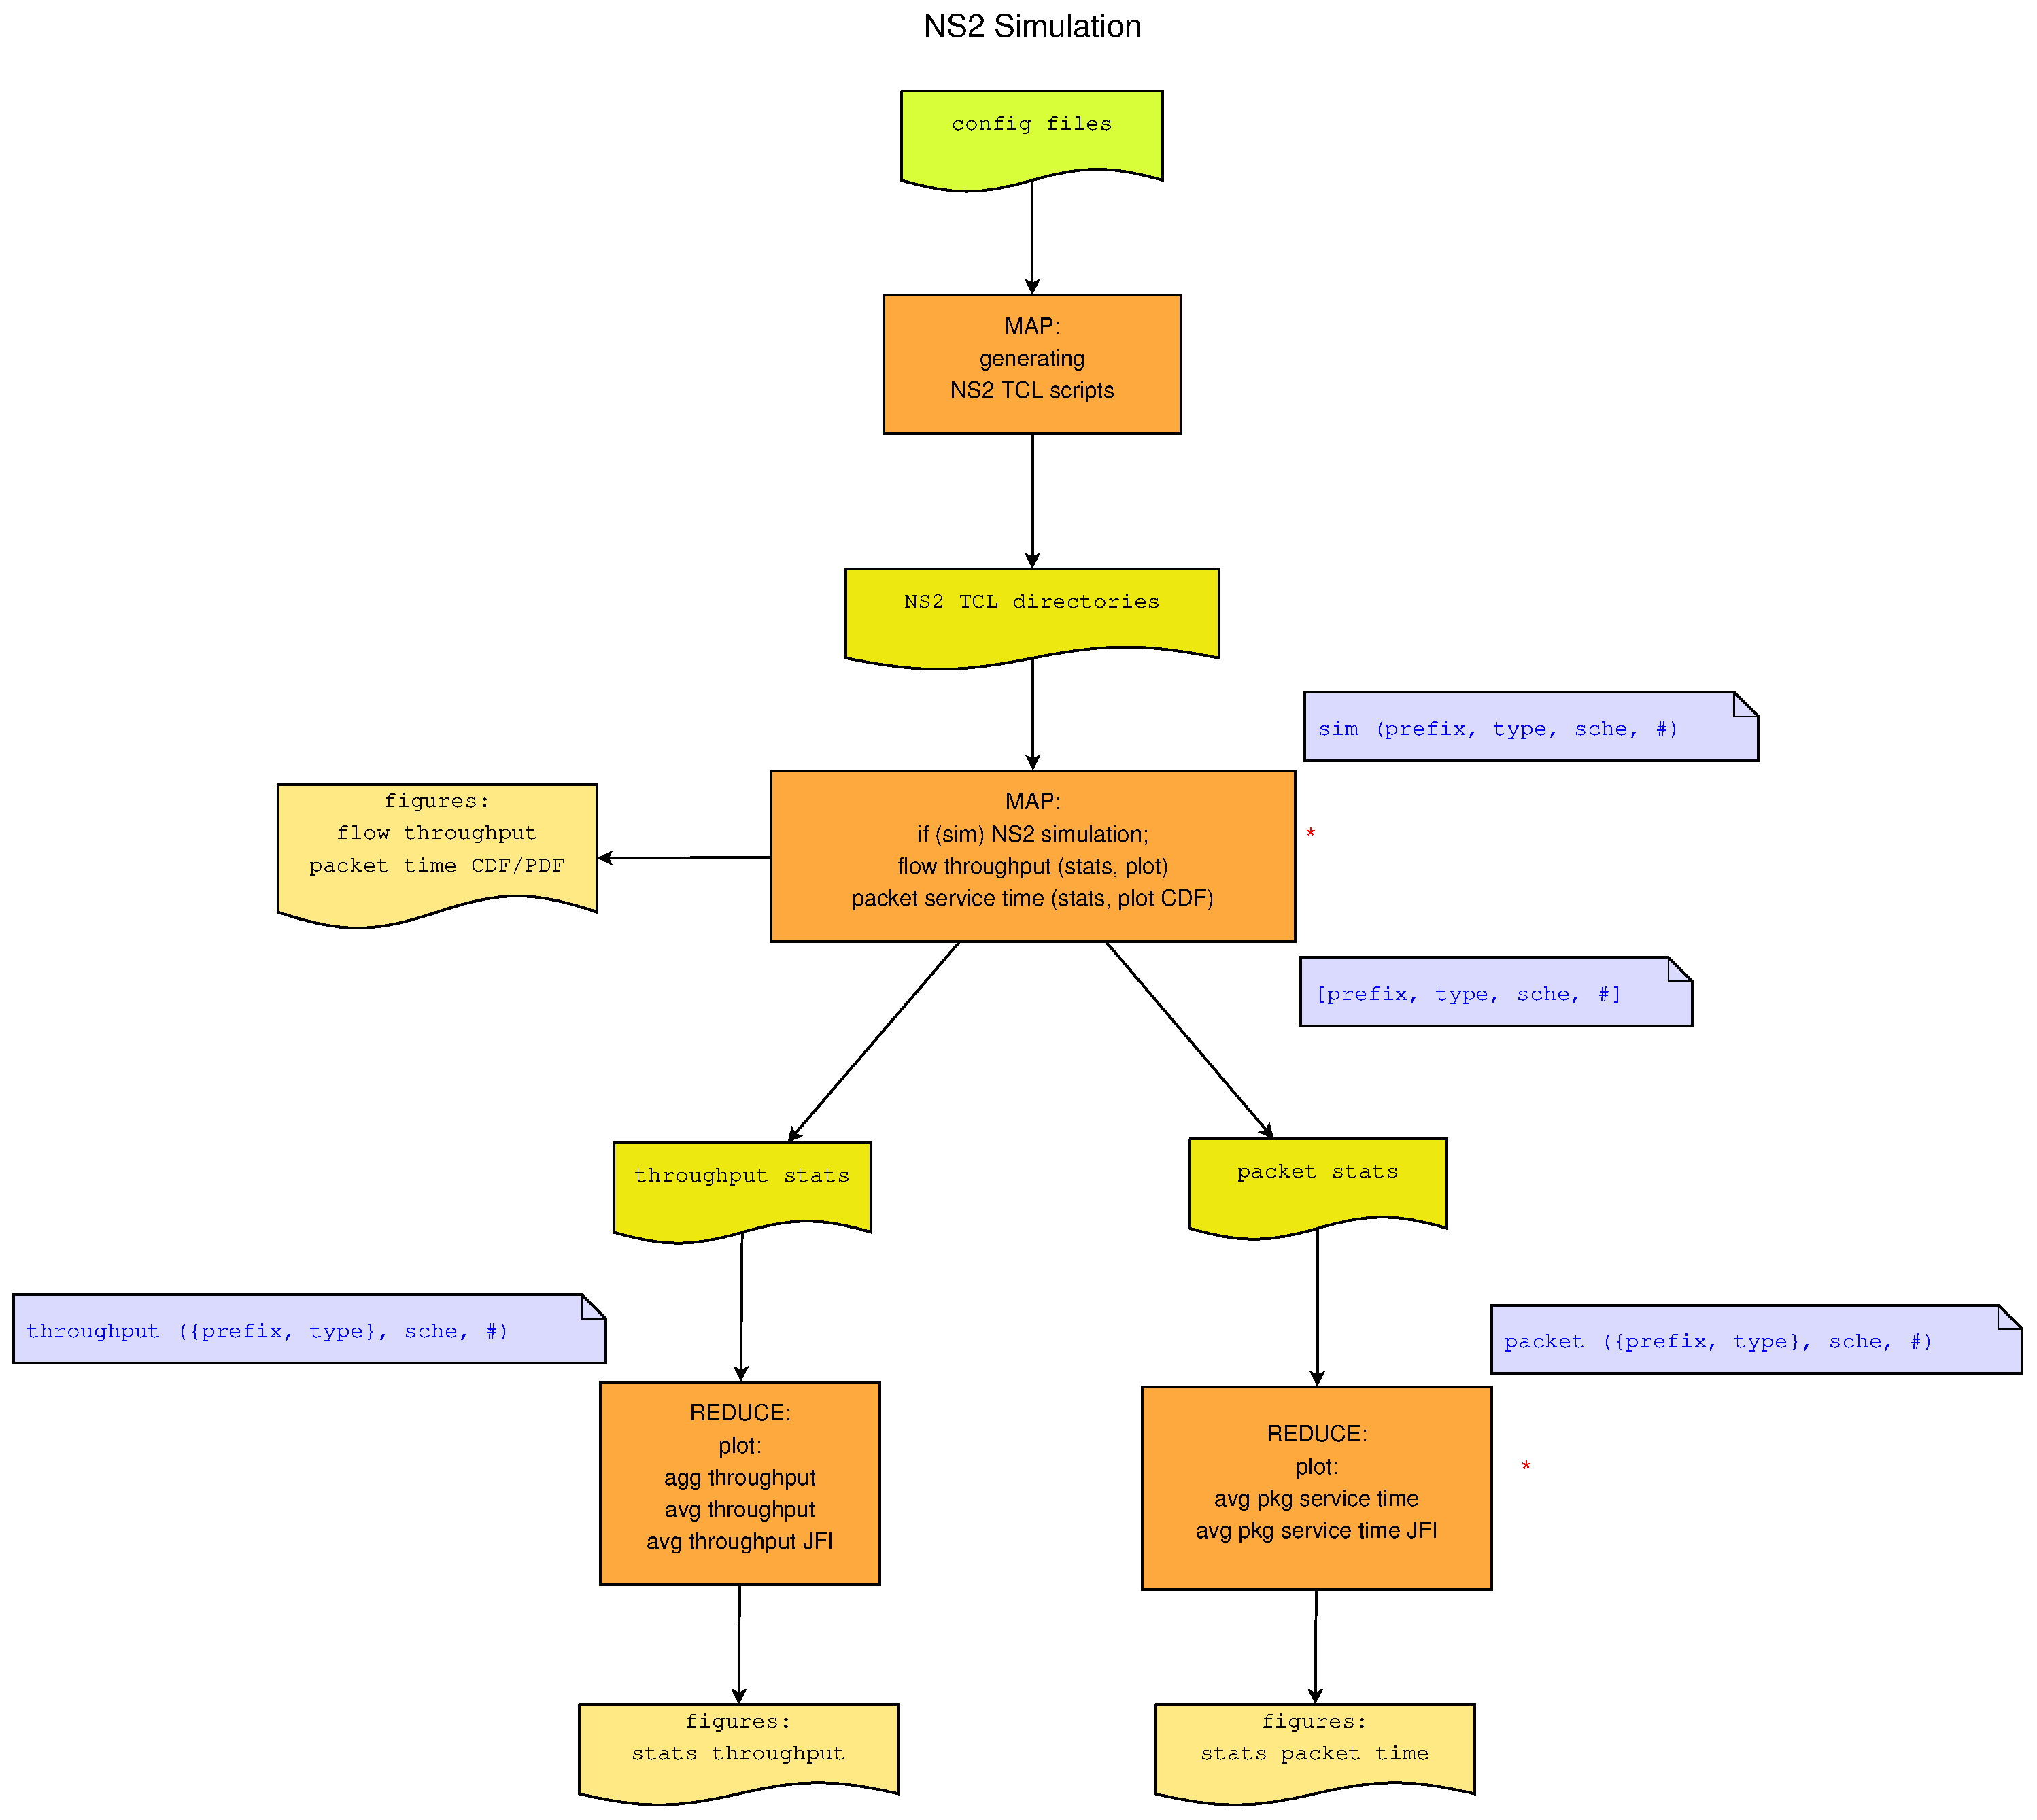
\includegraphics[height=0.8\textheight]{flowchart-mr-ns2sim}
%  \caption{The system.
%    The text in \fcolorbox{black}{vidtransoriginfile}{this color} is the original input file.
%    The text in \fcolorbox{black}{vidtranstmpfile}{this color} is the temp file.
%    The text in \fcolorbox{black}{vidtransfinalfile}{this color} is the final output file.
%    The text in \fcolorbox{black}{vidtransprocess}{this color} is process block.
%    The text in \fcolorbox{black}{vidtransfuncio}{\textcolor[HTML]{0000FF}{this color}} is the input/output of one process block.
%The process blocks signed by a \textcolor[HTML]{FF0000}{*} are the blocks cost most of the processing time.
%  }\label{fig:system}
\end{figure}

    \begin{itemize}
      \item 
      \item 
      \item 
    \end{itemize}
}




\section{Demo Project -- Media trans-coding}

\frame {
    \frametitle{Media trans-coding introduction}

    \begin{itemize}
      \item supports single host processing
      \item parallelize it by processing small chunk of video and merge them at the end of processing stage.
    \end{itemize}
}


\frame {
    \frametitle{Group Of Pictures (GOP)}

\begin{figure}\centering
  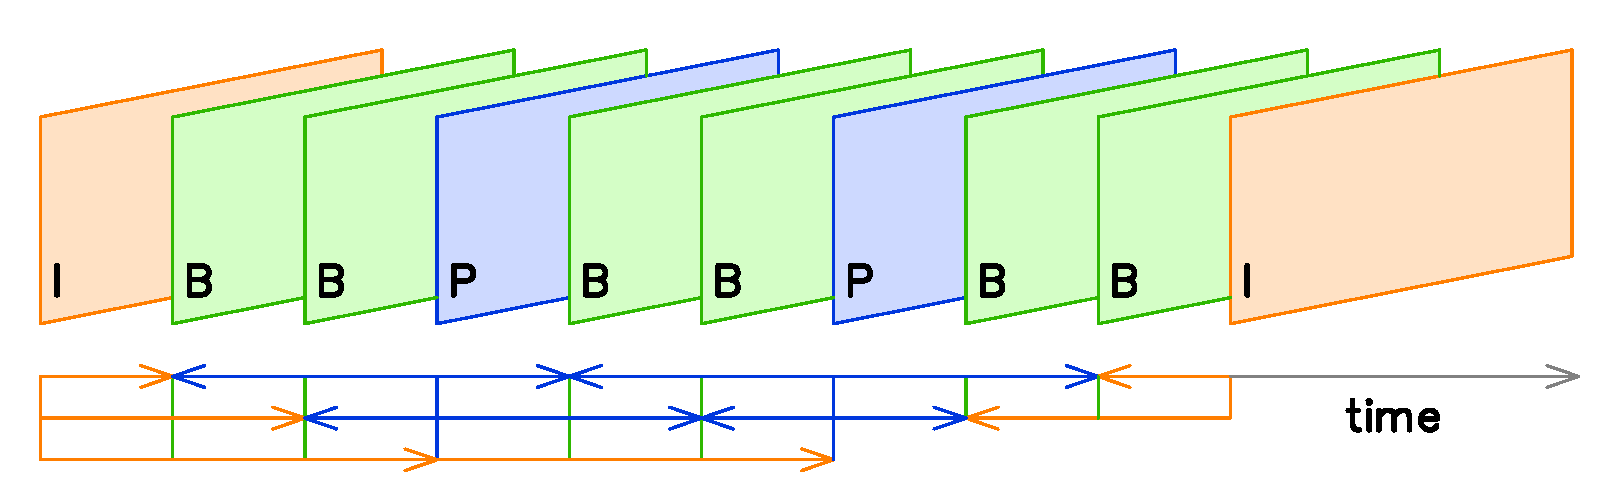
\includegraphics[width=0.7\textwidth]{gop-ipb.png}
  \caption{Example of a GOP structure (\href{http://en.wikipedia.org/wiki/Inter_frame}{Wikipedia}).}\label{fig:gopipb}
\end{figure}
An MPEG Group Of Pictures (GOP), starts with an "I" frame, follows with multiple "P" or "B" frames.
    \begin{itemize}
      \item "I" frame (Intra-coded picture, key frame) like a conventional static image file;
      \item "P" frame (Predicted picture) holds only the changes from the \emph{previous} frame;
      \item "B" frame (Bi-predictive picture) holds the differences between the current frame and both the preceding and following frames.
    \end{itemize}
}


\frame {
    \frametitle{Media trans-coding scenario}

    \begin{itemize}
      \item The input source, such as PNG sequences files, lossless video files, etc.
      \item The output format, such as DASH, H.264 etc.
    \end{itemize}
}


\frame {
    \frametitle{Media tran-scoding in MapReduce programming model}

\begin{figure}\centering
  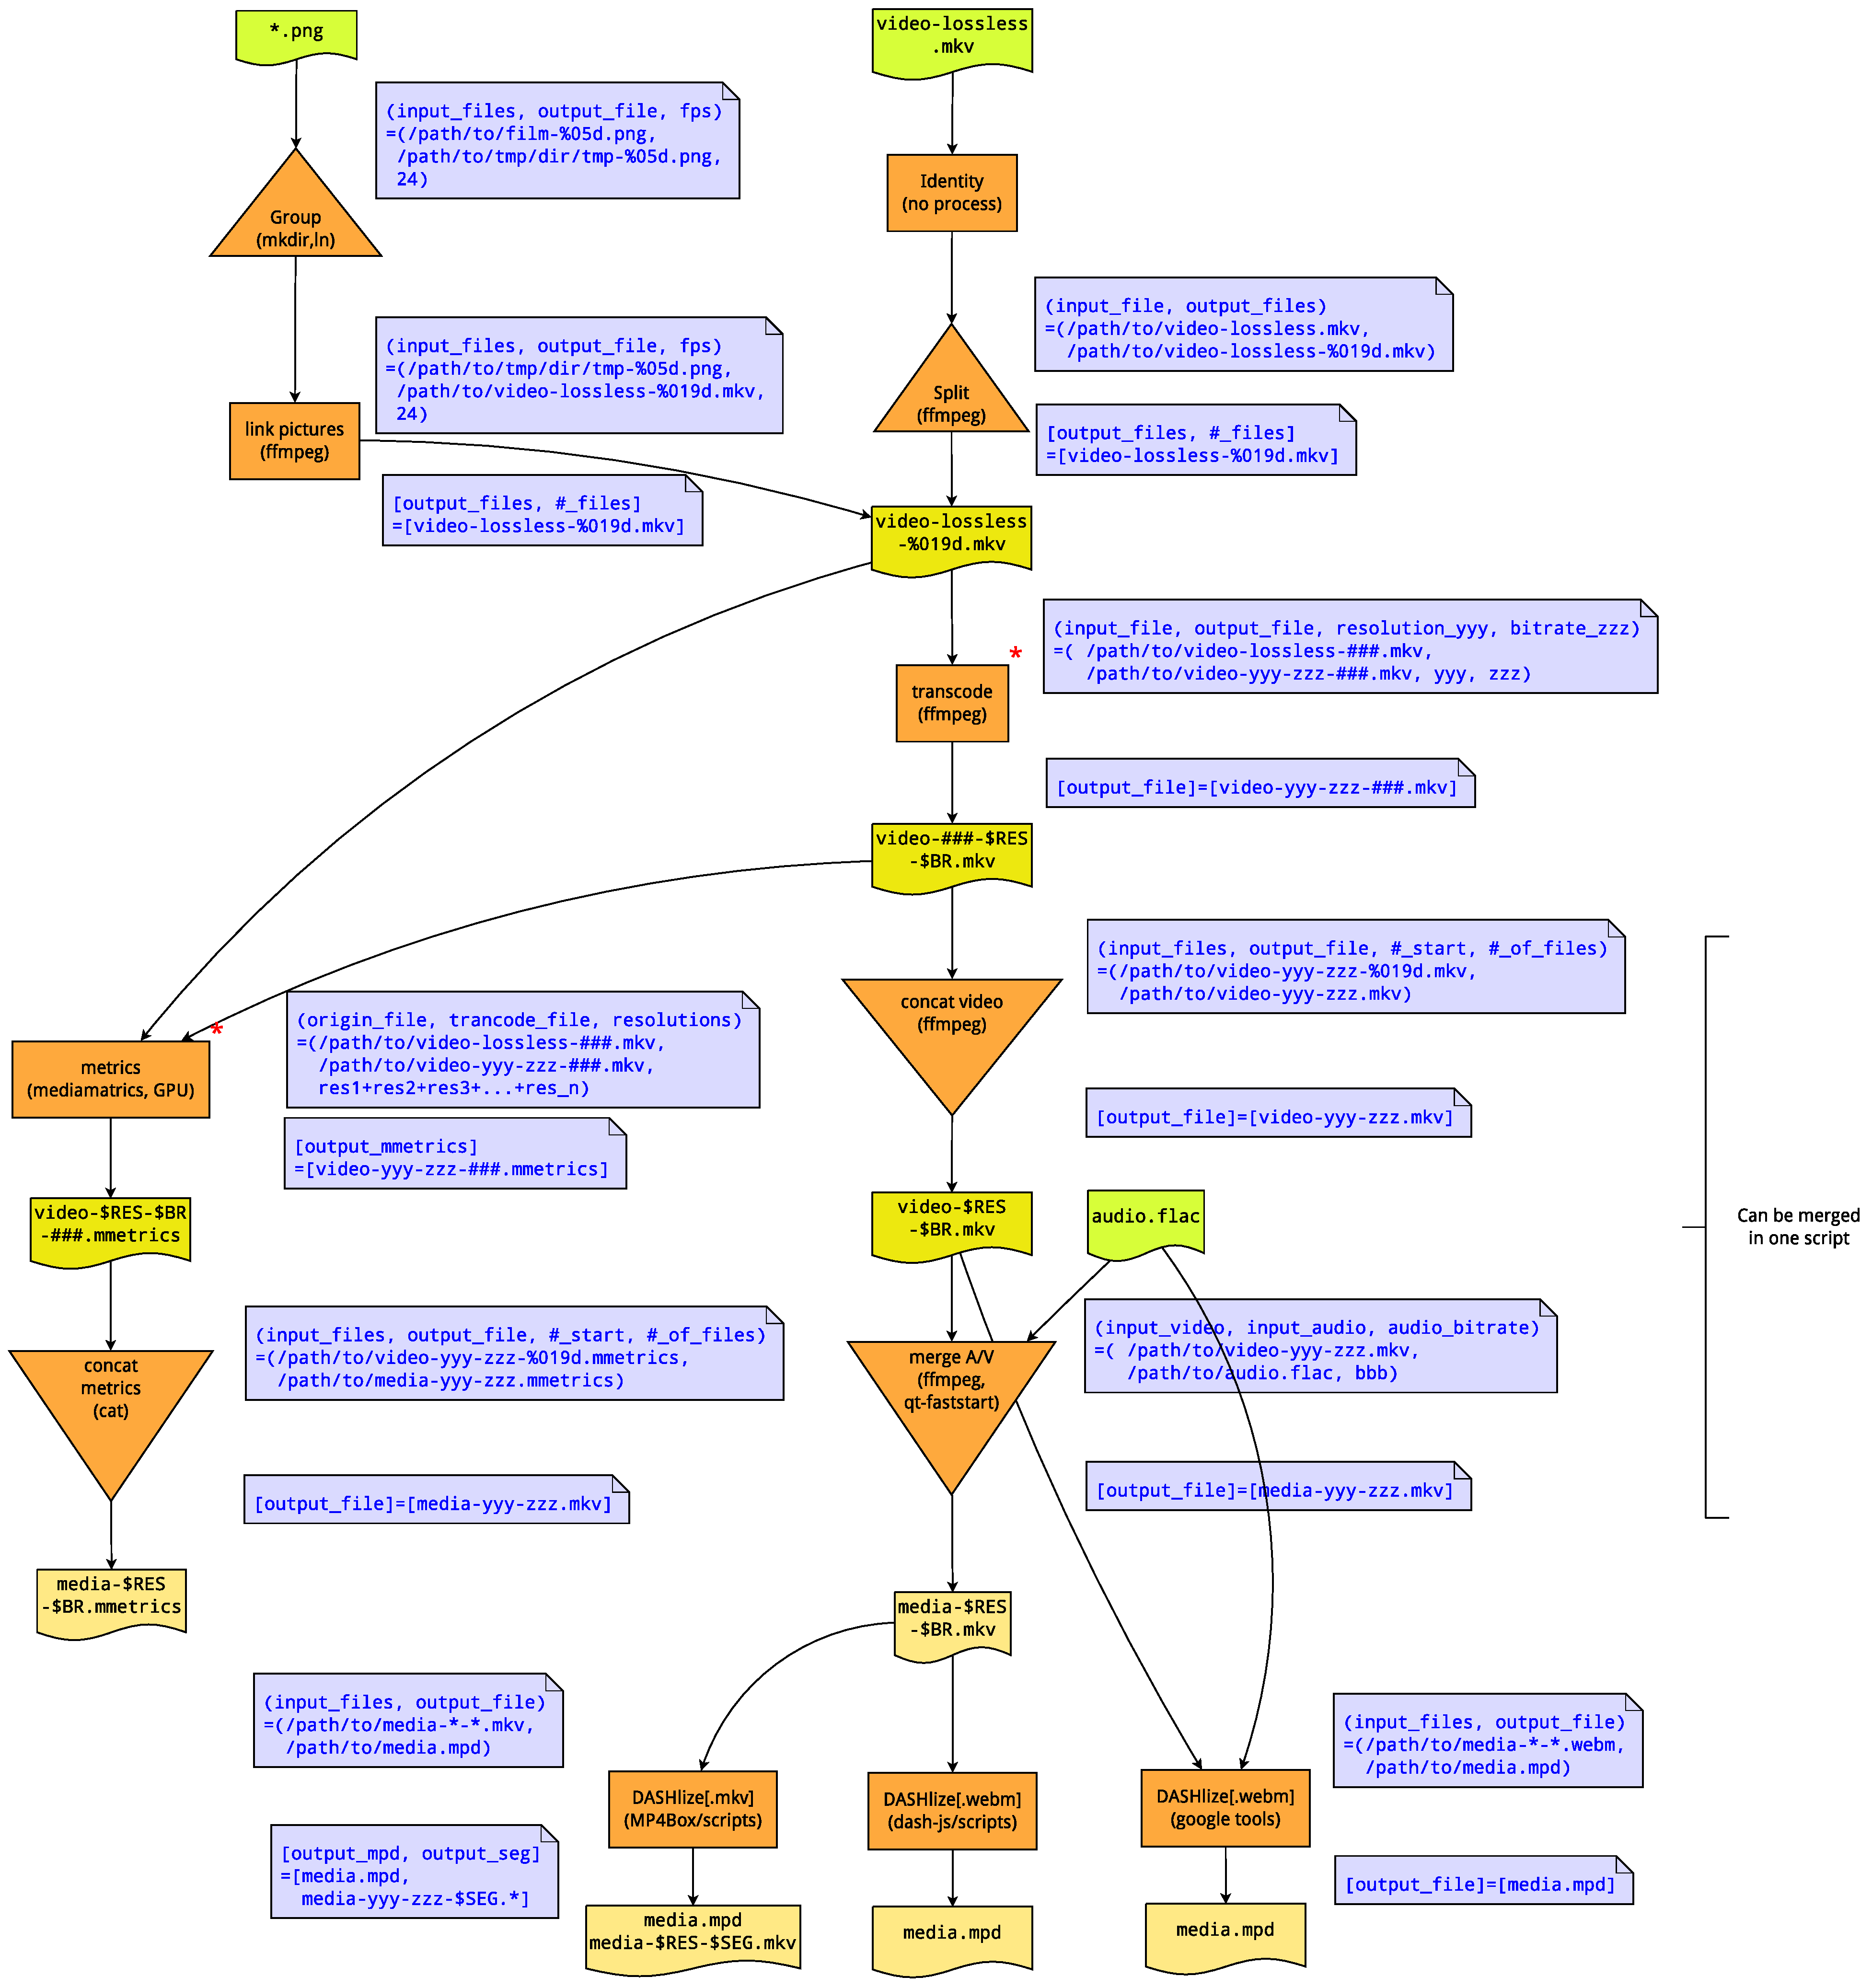
\includegraphics[height=0.8\textheight]{flowchart-mr-media-transcode}
%  \caption{The system.
%    The text in \fcolorbox{black}{vidtransoriginfile}{this color} is the original input file.
%    The text in \fcolorbox{black}{vidtranstmpfile}{this color} is the temp file.
%    The text in \fcolorbox{black}{vidtransfinalfile}{this color} is the final output file.
%    The text in \fcolorbox{black}{vidtransprocess}{this color} is process block.
%    The text in \fcolorbox{black}{vidtransfuncio}{\textcolor[HTML]{0000FF}{this color}} is the input/output of one process block.
%The process blocks signed by a \textcolor[HTML]{FF0000}{*} are the blocks cost most of the processing time.
%  }\label{fig:system}
\end{figure}

    \begin{itemize}
      \item 
      \item 
      \item 
    \end{itemize}
}


\end{document}
